 % @author nicolas.guelfi
% @date Tue Nov 05 17:26:22 CET 2013
%-------------------------------------------------------------------------------
% Copyright (c) 2013 University of Luxembourg.
% All rights reserved. This program and the accompanying materials
% are made available under the terms of the Eclipse Public License v1.0
% which accompanies this distribution, and is available at
% http://www.eclipse.org/legal/epl-v10.html
% 
% Contributors:
%     Alfredo Capozucca - initial API and implementation
%     Beno??t Ries - minor updates
%     Nicolas Guelfi - most content from messirbook
%-------------------------------------------------------------------------------

 
 
\documentclass[graybox,envcountchap,sectrefs]{svmono}  

%--------------------------------------------             
\hyphenation{abc-def-ghij-klm-nop-qrs-tuv-wxyz}
\usepackage{longtable}  % for tables spanning multiple pages
                      
                     
% for hyperrefs     
\usepackage[ps2pdf,
bookmarks=true,  
bookmarksnumbered=true, 
% true means bookmarks in
% left window are numbered
bookmarksopen=false,        
% true means only level 1
% are displayed.
colorlinks=true,
linkcolor=webblue]{hyperref}
\definecolor{webgreen}{rgb}{0, 0.5, 0} % less intense green
\definecolor{webblue}{rgb}{0, 0, 0.5} % less intense blue
\definecolor{webred}{rgb}{0.5, 0, 0} % less intense red
 
% for  quotes and smileys
\usepackage[english]{babel}
%--------------------------------------------
\usepackage{wasysym} 
% for track changes
%\usepackage[finalnew]{trackchanges}  
%\usepackage[finalold]{trackchanges}
%\usepackage[footnotes]trackchanges}
%\usepackage[margins]{trackchanges}
%\usepackage[margins, movemargins]{trackchanges}   
                  
\usepackage[inline]{trackchanges}
\addeditor{NG}
\addeditor{AC}
\addeditor{BR}  
 
%--------------------------------------------
\usepackage{upquote}
%\usepackage{url}
\usepackage{tabularx}
\usepackage{listings} 
\usepackage{enumerate}
\usepackage{longtable}

%--------------------------------------------
\usepackage[T1]{fontenc}
\usepackage{courier}
\usepackage{uncial}
\usepackage{ascii}
%--------------------------------------------
\usepackage{tocloft}

\usepackage[xindy,toc]{glossaries}
\renewcommand{\cftchapleader}{\cftdotfill{\cftsecdotsep}}
\makeglossaries
\renewcommand*\glspostdescription{\cftdotfill{\cftsecdotsep}}
 
\usepackage{makeidx}
\makeindex
  
%---------From Springer Sample------------------------------
\usepackage{multicol}        % used for the two-column index
\usepackage[bottom]{footmisc}% places footnotes at page bottom
%--------------------------------------------   
\usepackage{graphics}
\usepackage[dvipdfm]{geometry}
\usepackage{epsfig}
\usepackage{latexsym}
%--our packages
\usepackage{cite} 
\usepackage{listings}
\usepackage{verbatim}
\usepackage{spverbatim}
\usepackage{alltt}
\usepackage{MnSymbol}
%\usepackage{subfigure} % use for side-by-side figures
\usepackage{fancyvrb} 
\usepackage{amsmath}
%--------------------------------------------
\usepackage{asm} 
\usepackage{array}
\usepackage{graphicx}
%--------------------------------------------
%\geometry{hmargin=2.5cm, vmargin=3cm}
%--------------------------------------------
\newcounter{def} 
%--------------------------------------------
% to include pdf doc in the doc BUT only with pdflatex !!
\usepackage{datetime}
%\usepackage{appendix}
\usepackage{eso-pic,everyshi,ifthen,calc}
\usepackage[final]{pdfpages}
%\def\Remark{\noindent\textit{Remark : }} 
%--------------------------------------------
% For part/chapters table of contents
\usepackage{minitoc}  
%--------------------------------------------
% for nested relative paths in imported files
\usepackage{import}
%--------------------------------------------
%\usepackage{pdfsync}            
\usepackage{microtype}
%--------------------------------------------
%for french characters directly typed in French
\usepackage[utf8]{inputenc}
%--------------------------------------------
% For long words split
\usepackage{hyphenat}
\usepackage{xstring}
\usepackage{forloop}

\newsavebox\MyBreakChar%
\sbox\MyBreakChar{}% char to display the break after non char
\newsavebox\MySpaceBreakChar%
\sbox\MySpaceBreakChar{\hyp}% char to display the break after space
\makeatletter%
\newcommand*{\BreakableChar}[1][\MyBreakChar]{%
  \leavevmode%
  \prw@zbreak%
  \discretionary{\usebox#1}{}{}%
  \prw@zbreak%
}%
\makeatother

\newcounter{index}%
\newcommand{\AddBreakableChars}[1]{%
  \StrLen{#1 }[\stringLength]%
  \forloop[1]{index}{1}{\value{index}<\stringLength}{%
    \StrChar{#1}{\value{index}}[\currentLetter]%
    \IfStrEqCase{\currentLetter}{%
        % All the characters where you don't want hypen
        {,}{\currentLetter\BreakableChar[\MyBreakChar]}%
        {]}{\currentLetter\BreakableChar[\MyBreakChar]}
        {)}{\currentLetter\BreakableChar[\MyBreakChar]}%
        {-}{\currentLetter\BreakableChar[\MyBreakChar]}%
        {/}{\currentLetter\BreakableChar[\MyBreakChar]}%
        { }{\currentLetter\BreakableChar[\MyBreakChar]}%
        {[}{\currentLetter\BreakableChar[\MyBreakChar]}
        {(}{\currentLetter\BreakableChar[\MyBreakChar]}%        
        {a}{\currentLetter\BreakableChar[\MyBreakChar]}%
        {e}{\currentLetter\BreakableChar[\MyBreakChar]}%
        % All the charactes where a break should have a hypen
%        { }{\currentLetter\BreakableChar[\MySpaceBreakChar]}
%        {b}{\currentLetter\BreakableChar[\MySpaceBreakChar]}%
    }[\currentLetter]%
  }%
}%
  
%--------------------------------------------
% to change certain pages to landscape mode
\usepackage{pdflscape}    
%--------------------------------------------
% for Messir tables
\usepackage[table]{xcolor} 
%--------------------------------------------
% DOCUMENT BEGIN
%--------------------------------------------
\begin{document}

\newgeometry{textwidth=17cm,textheight=23.7cm} 


% Last Modification:
% @author AUTHOR_NAME
% @date TODAY_DATE


%  General Glossary
\newcommand{\glsict}{{information and communication technological}~}
 

% Messir General
\newcommand{\msrprolog}{{\emph Prolog}~} 
\newcommand{\msrmessir}{{\unclfamily Messir}~}
\newcommand{\msrexcalibur}{{\unclfamily Excalibur}~}
\newcommand{\msrmessim}{{\unclfamily MesSim}~}
\newcommand{\msrmessam}{{\unclfamily MessAm}~}
\newcommand{\msruml}{{\emph{UML}}~}
\newcommand{\msrcm}{\msrcode{{Concept Model}}~} 

\newcommand{\msrmessirmeth}{{\msrmessir}~methodology~}
\newcommand{\msrglsstyle}[1]{\emph{#1}}
\newcommand{\msrucname}[1]{\msrcode{\underline{#1}}}
\newcommand{\msrcode}[1]{{\ttfamily \hyphenchar\font=`\- #1}}


% Messir Lexique
\newcommand{\msrbool}{\msrcode{{\emph Boolean}}~}
\newcommand{\msrint}{\msrcode{{\emph Integer}}~}
\newcommand{\msrreal}{\msrcode{{\emph Real}}~}
\newcommand{\msrstring}{\msrcode{{\emph String}}~}
\newcommand{\msrenum}{\msrcode{{\emph enumeration}}~}
\newcommand{\msrenums}{\msrcode{{\emph enumerations}}~}



% Messir Analysis
\newcommand{\msrsysop}{\emph{system operation}}
\newcommand{\msrsysops}{\emph{system operations}}
\newcommand{\msrsysintpro}{\emph{system interaction protocol}}
\newcommand{\msrbhvmd}{\emph{system operation}}


%---------TABLES TEMPLATE--------------

%\rowcolors{2}{gray!20}{}

\newcounter{itemtable}


\newenvironment{usecase}{\begin{longtable}{|p{0.10\textwidth}
p{0.90\textwidth}|} \hline} {\hline \end{longtable}}


\newenvironment{usecaseinstance}{\begin{longtable}{|p{0.05\textwidth}
p{0.95\textwidth}|} \hline}
{\hline \end{longtable}}


\newenvironment{actortable}{
\begin{longtable}{|p{0.10\textwidth} p{0.90\textwidth}|}
\hline \hline}
{\hline \end{longtable}}


\newenvironment{datadictionary}{
\begin{longtable}{|p{0.15\textwidth} p{0.85\textwidth}|}
\hline \hline}
{\hline \end{longtable}}


\newenvironment{associationtypes}{
\begin{longtable}{|p{0.15\textwidth} p{0.85\textwidth}|}
\hline \hline}
{\hline \end{longtable}}


\newenvironment{operationmodel}{
\begin{longtable}{|p{0.10\textwidth} p{0.90\textwidth}|}
\hline \hline}
{\hline \end{longtable}}


\newenvironment{teststepmodel}{\begin{longtable}{|p{0.20\textwidth}|p{0.80\textwidth}|}
\hline}
{\hline \end{longtable}}


\newcommand*{\myfont}{\fontfamily{phv}\selectfont}


\newcommand\addheading[1]{
\hline
%\multicolumn{2}{|l|}{\cellcolor[gray]{0.9} \textbf{#1}} \\
\multicolumn{2}{|l|}{\textbf{\scshape #1}} \\
\hline \hline
\endfirsthead

\multicolumn{2}{@{}l}{\myfont{\bfseries\itshape{\ldots #1 table
continuation}}}\\
%\hline \hline 
%\multicolumn{2}{|l|}{\cellcolor[gray]{0.9} \textbf{#1}}\\
%\hline \hline
\endhead % all the lines above this will be repeated on every page

%\hline \hline
\multicolumn{2}{r@{}}{\myfont{\bfseries\itshape{continues in next page
\ldots}}}\\
\endfoot

\hline
\endlastfoot}

%\multicolumn{2}{|l|}{\cellcolor[gray]{0.8}
\newcommand\addrowheading[1]{
\hline \hline
\multicolumn{2}{|l|}{
	\setcounter{itemtable}{0}
 	\textbf{\itshape #1}}\\
\hline \hline
}


\newcommand\addsinglerow[1]{ 
\multicolumn{2}{|l|}{\begin{minipage}[t][][t]{1.0\textwidth}
#1 \end{minipage}} \\
%\hline
}


\newcommand\addsingletwocolumnrow[2]{ 
{\itshape #1} & #2 \\
%\hline
}


\newcommand\adddoublerow[2]{
\hline \hline
\multicolumn{2}{|l|}{\begin{minipage}[t][][t]{1.0\textwidth}
\textbf{\itshape #1} \end{minipage}} \\
\multicolumn{2}{|l|}{\begin{minipage}[t][][t]{1.0\textwidth}
#2 \end{minipage}} \\
\hline
}


\newcommand\adddoubletwocolumnrow[3]{ 
#1 & \textbf{#2} \\
& #3 \\
%\hline
}


\newcommand\addnumberedsinglerow[2]{
\stepcounter{itemtable} 
\text{#1 \theitemtable} & #2 \\
%\hline
}
 
 
\newcommand\addnumbereddoublerow[3]{
\stepcounter{itemtable} 
\text{#1 \theitemtable} & \textbf{#2} \\
		   & #3 \\
%\hline
}   



\newcommand\addalphanumberedsinglerow[2]{
\stepcounter{itemtable}
\text{#1 \alph{itemtable}} & #2 \\
%\hline
}
 
 
\newcommand\addalphanumbereddoublerow[3]{
\stepcounter{itemtable}
\text{#1 \alph{itemtable}} & \textbf{#2} \\
		   & #3 \\
%\hline
}

\input{doc/glossary/glossary.tex}
\newcommand{\msrprojectname}{\emph{icrash}~} 
\newcommand{\msricrash}{\emph{iCrash}~} 
  

%TITLE
%******************************************
\title{
\begin{tabular}{|>{\centering\arraybackslash\hspace{0pt}}p{16cm}|}
\hline
	\textbf{\msricrash:}\\
	\textbf{A Crisis Management Case Study}\\
	\textbf{\msrmessir Analysis Document}\\
	\textbf{ - v 1.1 - }\\
\hline
\end{tabular}
\vspace{2cm}}
 
%******************************************
\author{
\begin{tabular}{l}
		Laboratory for Advanced Software Systems\\
		University of Luxembourg\\
		6, rue R. Coudenhove-Kalergi, Luxembourg\\
\end{tabular}}

\date{\today~-~\currenttime}
%****************************************************


\maketitle
\newpage

%TOC
\setcounter{tocdepth}{2}  
\addtocounter{secnumdepth}{2}
\tableofcontents
\newpage

%TOF 
\listoffigures
\newpage

%TOL
\lstlistoflistings
\newpage

%DOCUMENT STRUCTURE
\input{doc/introduction/introduction.tex}
\newpage

\input{doc/general-description/general-description.tex}
\newpage

\input{doc-gen/doc-gen.tex}
\newpage

\input{doc/additional-constraints/additional-constraints.tex}
\newpage


%APPENDICES
\appendix
% Last Modification:
% @author Alexander
% @date 01/04/2014


\chapter{Use Case Description Tables}
\label{chap:APX-UseCaseDescriptionTables}

\section{Use cases list(s)}

\begin{itemize}
	\item Summary
	\begin{itemize}
		\item \msrucname{suDeployAndRun}
		\item \msrucname{suGlobalCrisisHandling}
	\end{itemize}
	\item user-goal
	\begin{itemize}
		\item \msrucname{ugAdministrateTheSystem}
		\item \msrucname{ugManageCrisis}
		\item \msrucname{ugMonitor}
		\item \msrucname{ugSecurelyUseSystem}
	\end{itemize}
	\item subfunction
	\begin{itemize}
		\item \msrucname{oeAddCoordinator}
		\item \msrucname{oeAlert}
		\item \msrucname{oeCloseAlert}
		\item \msrucname{oeCloseCrisis}
		\item \msrucname{oeCreateSystemAndEnvironment}
		\item \msrucname{oeDeleteCoordinator}
		\item \msrucname{oeGetAlertsSet}
		\item \msrucname{oeGetCrisisSet}
		\item \msrucname{oeSetCrisisHandler}
		\item \msrucname{oeInfoFam}
		\item \msrucname{oeLogin}
		\item \msrucname{oeLogout}
		\item \msrucname{oeReportOnCrisis}
		\item \msrucname{oeRequestEMSAssistance}
		\item \msrucname{oeReportEMSCrisisStatus}
		\item \msrucname{oeReplyToRequest}
		\item \msrucname{oeSetCrisisStatus}
		\item \msrucname{oeSollicitateCrisisHandling}
		\item \msrucname{oeValidateAlert}
	\end{itemize}
\end{itemize}
\newpage

\begin{itemize}
	\item \msrucname{suDeployAndRun}
		\begin{itemize}
			\item \msrucname{oeCreateSystemAndEnvironment}
			\item \msrucname{ugAdministrateTheSystem}
			\item \msrucname{suGlobalCrisisHandling}
			\item \msrucname{oeAlert}
		\end{itemize}
	\item \msrucname{suGlobalCrisisHandling}
		\begin{itemize}
			\item \msrucname{ugSecurelyUseSystem}
			\item \msrucname{ugMonitor}
			\item \msrucname{ugManageCrisis}
		\end{itemize}
	\item \msrucname{ugAdministrateTheSystem}
		\begin{itemize}
			\item \msrucname{ugSecurelyUseSystem}
			\item \msrucname{oeAddUser}
			\item \msrucname{oeDeleteUser}
		\end{itemize}
	\item \msrucname{ugSecurelyUseSystem}
		\begin{itemize}
		\item \msrucname{oeLogin}
		\item \msrucname{oeLogout}
		\end{itemize}
	\item \msrucname{ugManageCrisis}
		\begin{itemize} 
			\item \msrucname{oeSetCrisisStatus}
			\item \msrucname{oeSetCrisisHandler}
			\item \msrucname{oeReportOnCrisis}
			\item \msrucname{oeRequestEMSAssistance}
			\item \msrucname{oeCloseCrisis}
	\end{itemize}
	\item \msrucname{ugMonitor}
		\begin{itemize} 
			\item \msrucname{oeGetCrisisSet}
			\item \msrucname{oeValidateAlert}
			\item \msrucname{oeSollicitateCrisisHandling}
			
	\end{itemize}
\end{itemize} 

\newpage
\section{Use case Table(s)}

\subsection{Summary}
\clearpage
\begin{usecase}
  \addheading{Use-Case Description}
  \addsingletwocolumnrow{Name}{suDeployAndRun}
  \addsingletwocolumnrow{Scope}{System}
  \addsingletwocolumnrow{Altitude}{Summary}
  
  \addrowheading{Parameters}
  \addnumberedsinglerow{}{none}

  \addrowheading{Primary actor(s)}
  \addnumberedsinglerow{}{\msrcode{actAdministrator[active]}}
  
  \addrowheading{Secondary actor(s)}
  \addnumberedsinglerow{}{\msrcode{actMsrCreator[active]}}
  \addnumberedsinglerow{}{\msrcode{actCoordinator[active]}}
  \addnumberedsinglerow{}{\msrcode{actActivator[active]}}
  \addnumberedsinglerow{}{\msrcode{actComCompany[active]}}
  
  \addrowheading{Goal(s) description}
  \addsinglerow{The goal is to install the \msricrash system on its infrastructure and to exploit its capacities related to the secure administration and efficient handling of car crash crisis situations depending on alerts received.}
  
  \addrowheading{Reuse}
  \addnumberedsinglerow{}{\msrucname{oeCreateSystemAndEnvironment}}
  \addnumberedsinglerow{}{\msrucname{ugAdministrateTheSystem}[1..*]}
  \addnumberedsinglerow{}{\msrucname{suGlobalCrisisHandling}[1..*]}
  \addnumberedsinglerow{}{\msrucname{oeSetClock}[1..*]}
  \addnumberedsinglerow{}{\msrucname{oeSollicitateCrisisHandling}[*]}
  \addnumberedsinglerow{}{\msrucname{oeAlert}[1..*]}
  
  \addrowheading{Protocol condition(s)}
  \addnumberedsinglerow{}{the \msricrash system has never been deployed and used}
  
  \addrowheading{Pre-condition(s)}
  \addnumberedsinglerow{}{none}
  
  \addrowheading{Main post-condition(s)}
  \addnumberedsinglerow{}{\msricrash system has been created and has handled the crisis situations for which it received alerts through the communication company.}
  
  \addrowheading{Main success steps}
  \addalphanumberedsinglerow{}{the actor \msrcode{actMsrCreator} executes the \msrucname{oeCreateSystemAndEnvironment} use case}
  \addalphanumberedsinglerow{}{the actor \msrcode{actAdministrator} executes the \msrucname{ugAdministrateTheSystem} use case}
  \addalphanumberedsinglerow{}{the actor \msrcode{actComCompany} executes the \msrucname{oeAlert} use case}
  \addalphanumberedsinglerow{}{the actor \msrcode{actActivator} executes the \msrucname{oeSetClock} }
  \addalphanumberedsinglerow{}{the actor \msrcode{actActivator} executes the \msrucname{oeSollicitateCrisisHandling}}
  \addalphanumberedsinglerow{}{the actor \msrcode{actCoordinator} executes the \msrucname{suGlobalCrisisHandling} use case}
  
  \addrowheading{Step Constraints Ordering and Extensions}
  \addnumberedsinglerow{}{step (a) must be always the first step.}
  \addnumberedsinglerow{}{step (b) (c) (d) (e) and (f) executions are interleaved.}
  \addnumberedsinglerow{}{step (b) (c) (d) (e) and (f) can be executed multiple times.}
  \addnumberedsinglerow{}{step (f) can be executed by different \msrcode{actCoordinator} actors.}
  \addnumberedsinglerow{}{step (f) can be executed as a reaction to step (e).}
  
  \addrowheading{Additional Information}
  \addsinglerow{none}
\end{usecase} 

\clearpage

\begin{figure}[htbp]
\begin{center}
\scalebox{0.95}{
\includegraphics[width=180mm]{./images/iCrash-UseCase-suDeployAndRun-Diagram.eps} 
\normalsize}
\end{center}
\caption[\msricrash Use Case Diagram: suDeployAndRun]{\msricrash Use Case Diagram: suDeployAndRun}
\label{fig:icrash-RE-UCD-suDeployAndRun}
\end{figure}
\vspace{0.5cm}

\clearpage

\begin{usecase}
  \addheading{Use-Case Description}
  \addsingletwocolumnrow{Name}{suGlobalCrisisHandling}
  \addsingletwocolumnrow{Scope}{System}
  \addsingletwocolumnrow{Altitude}{Summary}
  
  \addrowheading{Parameters}
  \addnumberedsinglerow{}{none}
  
  \addrowheading{Primary actor(s)}
  \addnumberedsinglerow{}{\msrcode{actCoordinator[active]}
	}
  \addrowheading{Secondary actor(s)}
  \addnumberedsinglerow{}{none}
  
  \addrowheading{Goal(s) description}
  \addsinglerow{the \msrcode{actCoordinator}'s goal is to monitor the alerts received and the corresponding crisis in order to act as necessary to handle all the crisis.}
  
  \addrowheading{Reuse}
  \addnumberedsinglerow{}{\msrucname{ugSecurelyUseSystem}[1..*]}
  \addnumberedsinglerow{}{\msrucname{ugMonitor}[1..*]}
  \addnumberedsinglerow{}{\msrucname{ugManageCrisis}[1..*]}
  
  \addrowheading{Protocol condition(s)}
  \addnumberedsinglerow{}{the \msricrash system has been deployed}
  \addnumberedsinglerow{}{the coordinator actor involved in the use case has been declared by the actor \msrcode{actAdministrator}.}
  
  \addrowheading{Pre-condition(s)}
  \addnumberedsinglerow{}{none}
  
  \addrowheading{Main post-condition(s)}
  \addnumberedsinglerow{}{modifications has been made by the coordinator on existing alerts or crisis
  \newline OR the coordinator requested an updated status on existing alerts or crisis.}
  
  \addrowheading{Main success steps}
  \addalphanumberedsinglerow{}{the actor \msrcode{actCoordinator} executes the \msrucname{ugSecurelyUseSystem} use case}
  \addalphanumberedsinglerow{}{the actor \msrcode{actCoordinator} executes the \msrucname{ugMonitor} use case}
  \addalphanumberedsinglerow{}{the actor \msrcode{actCoordinator} executes the \msrucname{ugManageCrisis} use case}

  \addrowheading{Step Constraints Ordering and Extensions}
  \addnumberedsinglerow{}{steps (a) (b) and (c) executions are interleaved (steps (b) and (c) have there protocol constrained by steps of (a)).}
  \addnumberedsinglerow{}{steps (a) (b) and (c) can be executed multiple times.}
  
  \addrowheading{Additional Information}
  \addsinglerow{there might be several actors \msrcode{actCoordinator} that concurrently execute their \msrcode{suGlobalCrisisHandling} use cases.}
\end{usecase}


\clearpage 

\begin{figure}[htbp]
\begin{center}
\scalebox{0.95}{
\includegraphics[width=180mm]{./images/iCrash-UseCase-suGlobalCrisisHandling-Diagram.eps} 
\normalsize}
\end{center}
\caption[\msricrash Use Case Diagram: suGlobalCrisisHandling]{\msricrash Use Case Diagram: suGlobalCrisisHandling}
\label{fig:icrash-RE-UCD-suGlobalCrisisHandling}
\end{figure}
\vspace{0.5cm}


\subsection{User-goal}
\clearpage

\begin{usecase}
  \addheading{Use-Case Description}
  \addsingletwocolumnrow{Name}{ugAdministrateTheSystem}
  \addsingletwocolumnrow{Scope}{System}
  \addsingletwocolumnrow{Altitude}{Summary}
  
  \addrowheading{Parameters}
  \addnumberedsinglerow{}{none}
  
  \addrowheading{Primary actor(s)}
  \addnumberedsinglerow{}{\msrcode{actAdministrator[active]}}
   
  \addrowheading{Secondary actor(s)}
  \addnumberedsinglerow{}{none}
  
  \addrowheading{Goal(s) description}
  \addsinglerow{the \msrcode{actAdministrator}'s goal is to follow an identification procedure to be allowed to add or delete the necessary crisis coordinators that will be granted the responsibility to handle alerts and crisis.}
  
  \addrowheading{Reuse}
  \addnumberedsinglerow{}{\msrucname{ugSecurelyUseSystem}[1..*]}
  \addnumberedsinglerow{}{\msrucname{oeAddUser}[1..*]}
  \addnumberedsinglerow{}{\msrucname{oeDeleteUser}[1..*]}
  
  \addrowheading{Protocol condition(s)}
  \addnumberedsinglerow{}{the \msricrash system has been deployed.}
  
  \addrowheading{Pre-condition(s)}
  \addnumberedsinglerow{}{none}
  
  \addrowheading{Main post-condition(s)}
  \addnumberedsinglerow{}{a new user is added to the system and can now
  securely use the system.}
  
  \addrowheading{Main success steps}
  \addalphanumberedsinglerow{}{the actor \msrcode{actAdministrator} executes the \msrucname{ugSecurelyUseSystem} use case.}
  \addalphanumberedsinglerow{}{the actor \msrcode{actAdministrator} executes the
  \msrucname{oeAddUser} use case.}
  \addalphanumberedsinglerow{}{the actor \msrcode{actAdministrator} executes the
  \msrucname{oeDeleteUser} use case.}
  
  \addrowheading{Step Constraints Ordering and Extensions}
  \addnumberedsinglerow{}{steps (a) (b) and (c) executions are interleaved (steps (b) and (c) have there protocol constrained by steps of (a)).}
  \addnumberedsinglerow{}{steps (a) (b) and (c) can be executed multiple times.}
  
  \addrowheading{Additional Information}
  \addsinglerow{none}
\end{usecase}

 \clearpage

 \begin{figure}[htbp]
 \begin{center} 
 \scalebox{0.95}{
 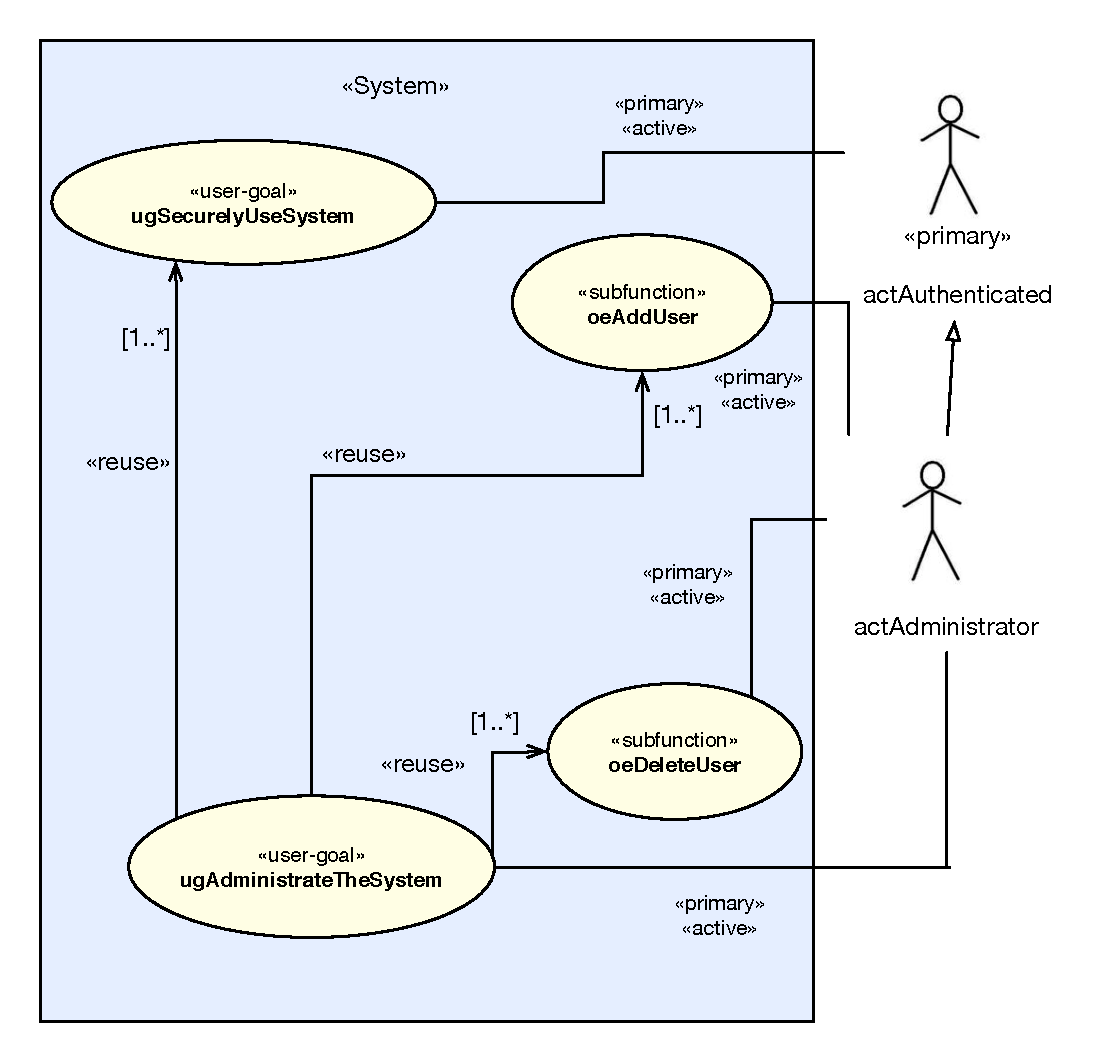
\includegraphics[width=180mm]{./images/ugAdministrateTheSystem.eps}
 \normalsize}
 \end{center}
 \caption[\msricrash Use Case Diagram:  ugAdministrateTheSystem Diagram]{\msricrash Use Case Diagram:  ugAdministrateTheSystem}
 \label{fig:icrash-RE-UCD- ugAdministrateTheSystem}
 \end{figure}
 \vspace{0.5cm}
\clearpage

\begin{usecase}
  \addheading{Use-Case Description}
  \addsingletwocolumnrow{Name}{ugSecurelyUseSystem}
  \addsingletwocolumnrow{Scope}{System}
  \addsingletwocolumnrow{Altitude}{user-goal}

  \addrowheading{Parameters}
  \addnumberedsinglerow{}{none}
  
  \addrowheading{Primary actor(s)}
  \addnumberedsinglerow{}{\msrcode{actAuthenticated[abstract]}}
  
  \addrowheading{Secondary actor(s)}
  \addnumberedsinglerow{}{none}

  \addrowheading{Goal(s) description}
  \addsinglerow{the goal is to follow an identification procedure and thus be
  allowed to safely use the system and it's features.}
  
  \addrowheading{Reuse}
  \addnumberedsinglerow{}{\msrucname{oeLogin}}
  \addnumberedsinglerow{}{\msrucname{oeLogout}}
  
  \addrowheading{Protocol condition(s)}
  \addnumberedsinglerow{}{the \msricrash system has been deployed.}
  \addnumberedsinglerow{}{the a useraccount has been created for the user
  trying to securely use the system.}
  
  \addrowheading{Pre-condition(s)}
  \addnumberedsinglerow{}{none}
  
  \addrowheading{Main post-condition(s)}
  \addnumberedsinglerow{}{the \msrcode{actAuthenticated} is known by the system not to be logged.}
  
  \addrowheading{Main success steps}
  \addalphanumberedsinglerow{}{the actor \msrcode{actAuthenticated} executes the \msrucname{oeLogin} use case.}
  \addalphanumberedsinglerow{}{the actor \msrcode{actAuthenticated} executes the \msrucname{oeLogout} use case}
  
  \addrowheading{Step Constraints Ordering and Extensions}
  \addnumberedsinglerow{}{step (a) must always precede step (b).}
 
  \addrowheading{Additional Information}
  \addsinglerow{none.}
\end{usecase}

\clearpage

\begin{figure}[htbp] 
\begin{center} 
\scalebox{0.95}{
\includegraphics[width=180mm]{./images/iCrash-UseCase-ugSecurelyUseSystem-Diagram.eps} 
\normalsize}
\end{center}
\caption[\msricrash Use Case Diagram:  ugAdministrateTheSystem Diagram]{\msricrash Use Case Diagram:  ugAdministrateTheSystem}
\label{fig:icrash-RE-UCD- ugAdministrateTheSystem} 
\end{figure}
\vspace{0.5cm}


\clearpage

\begin{usecase}
  \addheading{Use-Case Description}
  \addsingletwocolumnrow{Name}{ugManageCrisis}
  \addsingletwocolumnrow{Scope}{System}
  \addsingletwocolumnrow{Altitude}{Summary}
  
  \addrowheading{Parameters}
  \addnumberedsinglerow{}{none}

  \addrowheading{Primary actor(s)}
  \addnumberedsinglerow{}{\msrcode{\msrcode{actCoordinator[active]}}}
  
  \addrowheading{Secondary actor(s)}
  \addnumberedsinglerow{}{none.}
  
  \addrowheading{Goal(s) description}
  \addsinglerow{The goal is to do an action that makes the handling of a crisis or an alert progress.}
  
  \addrowheading{Reuse}
  \addnumberedsinglerow{}{\msrucname{oeValidateAlert}}
  \addnumberedsinglerow{}{\msrucname{oeSetCrisisStatus}}
  \addnumberedsinglerow{}{\msrucname{oeSetCrisisHandler}}
  \addnumberedsinglerow{}{\msrucname{oeReportOnCrisis}}
  \addnumberedsinglerow{}{\msrucname{oeCloseCrisis}}
  \addnumberedsinglerow{}{\msrucname{oeCloseAlert}}
  
 \addrowheading{Protocol condition(s)}
  \addnumberedsinglerow{}{the \msricrash system is started}
  
  \addrowheading{Pre-condition(s)}
  \addnumberedsinglerow{}{none}
  
  \addrowheading{Main post-condition(s)}
  \addnumberedsinglerow{}{there exist one alert or one crisis whose related information has been changed.}
  
  \addrowheading{Main success steps}
  \addalphanumberedsinglerow{}{the actor \msrcode{actCoordinator} executes the \msrucname{oeValidateAlert} use case.}
  \addalphanumberedsinglerow{}{the actor \msrcode{actCoordinator} executes the \msrucname{oeSetCrisisStatus} use case.}
  \addalphanumberedsinglerow{}{the actor \msrcode{actCoordinator} executes the \msrucname{oeSetCrisisHandler} use case.}
  \addalphanumberedsinglerow{}{the actor \msrcode{actCoordinator} executes the \msrucname{oeReportOnCrisis} use case.}
  \addalphanumberedsinglerow{}{the actor \msrcode{actCoordinator} executes the \msrucname{oeCloseCrisis} use case.}
  \addalphanumberedsinglerow{}{the actor \msrcode{actCoordinator} executes the \msrucname{oeCloseAlert} use case.}
  
  \addrowheading{Step Constraints Ordering and Extensions}
  \addnumberedsinglerow{}{managing a crisis is doing one of the indicated use cases.}
\end{usecase}

\clearpage

\begin{figure}[htbp]
\begin{center}
\scalebox{0.95}{
\includegraphics[width=180mm]{./images/iCrash-UseCase-ugManageCrisis-Diagram.eps} 
\normalsize}
\end{center}
\caption[\msricrash Use Case Diagram: suDeployAndRun]{\msricrash Use Case Diagram: suDeployAndRun}
\label{fig:icrash-RE-UCD-suDeployAndRun}
\end{figure}
\vspace{0.5cm}


\subsection{Subfunction}
\clearpage

\begin{usecase}
  \addheading{Use-Case Description}
  \addsingletwocolumnrow{Name}{oeSollicitateCrisisHandling}
  \addsingletwocolumnrow{Scope}{System}
  \addsingletwocolumnrow{Altitude}{subfunction}
  
  \addrowheading{Parameters}
  \addnumberedsinglerow{}{none}
  
  \addrowheading{Primary actor(s)}
  \addnumberedsinglerow{}{\msrcode{actActivator[active]}}
  
  \addrowheading{Secondary actor(s)}
  \addnumberedsinglerow{}{\msrcode{actAdministrator[passive]}}
  \addnumberedsinglerow{}{\msrcode{actCoordinator[passive,multiple]}}
   
  \addrowheading{Goal(s) description}
  \addsinglerow{the \msrcode{actActivator}'s goal is to decrease the number of unhandled crisis.}
  
  \addrowheading{Reuse}
  \addnumberedsinglerow{}{none}
  
  \addrowheading{Protocol condition(s)}
  \addnumberedsinglerow{}{the \msricrash system has been deployed.}
  \addnumberedsinglerow{}{there exist some crisis still pending and for which no solicitation has been sent to the administrator and the coordinators for more than a predefined maximum delay.}
  
  \addrowheading{Pre-condition(s)}
  \addnumberedsinglerow{}{none}
  
  \addrowheading{Main post-condition(s)}
  \addnumberedsinglerow{}{a simple text message \msrcode{ieMessage('There are alerts not treated since more than the defined delay. Please REACT !')} is sent to the system administrator and to all the coordinators of the environment for each crisis that is known to be not handled and for which no solicitation has been sent to the administrator and the coordinators for more than a predefined maximum delay.}
  \addnumberedsinglerow{}{the reminder period for the concerned crisis is initialized.}
  
  \addrowheading{Main success steps}
  \addalphanumberedsinglerow{}{the actor \msrcode{actActivator} sends the message \msrucname{oeSollicitateCrisisHandling()} to the system.}
  
  \addrowheading{Step Constraints Ordering and Extensions}
  \addnumberedsinglerow{}{none.}
  
  \addrowheading{Additional Information}
  \addsinglerow{none}
\end{usecase}

\clearpage

\begin{figure}[htbp] 
\begin{center} 
\scalebox{0.95}{

\includegraphics[width=180mm]{./images/iCrash-UseCase-oeSollicitateCrisisHandling-Diagram.eps} 
\normalsize}
\end{center}
\caption[\msricrash Use Case Diagram:  oeSollicitateCrisisHandling Diagram]{\msricrash Use Case Diagram:  oeSollicitateCrisisHandling}
\label{fig:icrash-RE-UCD- oeSollicitateCrisisHandling} 
\end{figure}
\vspace{0.5cm}


\clearpage

\begin{usecase}
  \addheading{Use-Case Description}
  \addsingletwocolumnrow{Name}{oeCloseCrisis}
  \addsingletwocolumnrow{Scope}{System}
  \addsingletwocolumnrow{Altitude}{subfunction}
  
  \addrowheading{Parameters}
  \addnumberedsinglerow{}{\msrcode{crisisID:dtCrisisID} - the crisis identification}
  
  \addrowheading{Primary actor(s)}
  \addnumberedsinglerow{}{\msrcode{actCoordinator[active]}}
  
  \addrowheading{Secondary actor(s)}
  \addnumberedsinglerow{}{\msrcode{actComCompany[passive]}}
  
  \addrowheading{Goal(s) description}
  \addsinglerow{the \msrcode{actCoordinator}'s goal is to declare a crisis as closed.}
  
  \addrowheading{Reuse}
  \addnumberedsinglerow{}{none}

  \addrowheading{Protocol condition(s)}
  \addnumberedsinglerow{}{the \msricrash system has been deployed.
}
  \addrowheading{Pre-condition(s)}
  \addnumberedsinglerow{}{none}
  
  \addrowheading{Main post-condition(s)}
  \addnumberedsinglerow{}{the crisis is known by the system to be closed.}
  \addnumberedsinglerow{}{a message \msrcode{ieSmsSend(AdtPhoneNumber,AdtComment)} is sent to the \msrcode{actComCompany} actor for each registered alert declared by a SMS coming from phone number \msrcode{AdtPhoneNumber} and related to the crisis \msrcode{crisisID}. All the messages have the same textual message \msrcode{AdtComment} giving them the minimal information on the crisis they alerted.}
  
  \addrowheading{Main success steps}
  \addalphanumberedsinglerow{}{the actor \msrcode{actCoordinator} sends the message \msrucname{oeCloseCrisis(crisisID)} to the system.}
  
  \addrowheading{Step Constraints Ordering and Extensions}
  \addnumberedsinglerow{}{none}
  
  \addrowheading{Additional Information}
  \addsinglerow{none}
  
\end{usecase} 

\clearpage

\begin{figure}[htbp] 
\begin{center} 
\scalebox{0.95}{

\includegraphics[width=180mm]{./images/iCrash-UseCase-oeCloseCrisis-Diagram.eps} 
\normalsize}
\end{center}
\caption[\msricrash Use Case Diagram:  oeCloseCrisis Diagram]{\msricrash Use Case Diagram:  oeCloseCrisis}
\label{fig:icrash-RE-UCD- oeCloseCrisis} 
\end{figure}
\vspace{0.5cm}
\newpage

\begin{usecase}
  \addheading{Use-Case Description}
  \addsingletwocolumnrow{Name}{oeAddUser}
  \addsingletwocolumnrow{Scope}{System}
  \addsingletwocolumnrow{Altitude}{subfunction}
   
  \addrowheading{Parameters}
  \addnumberedsinglerow{}{\msrcode{CoodrinatorID:dtCrisisID} - the
  Coordinator's identification}
  \addnumberedsinglerow{}{\msrcode{Login:dtLogin} - the username of the
  Coordinator}
  \addnumberedsinglerow{}{\msrcode{Password:dtPassword} - the password of the
  Coordinator}
  \addnumberedsinglerow{}{\msrcode{Usertyep:etUserType} - the Type of user
  [Coordinator, DomainExpert or EMS]}
  
  \addrowheading{Primary actor(s)}
  \addnumberedsinglerow{}{\msrcode{actAdministrator[active]}}
  
  \addrowheading{Secondary actor(s)}
  \addnumberedsinglerow{}{\msrcode{actCoordinator[passive]}}
  \addnumberedsinglerow{}{\msrcode{actDomainExpert[passive]}}
  \addnumberedsinglerow{}{\msrcode{actEMS[passive]}}
  
  \addrowheading{Goal(s) description}
  \addsinglerow{the \msrcode{actAdministrator}'s goal is to add
  new user to the system so he/she can safely use the
  system.}
  
  \addrowheading{Reuse}
  \addnumberedsinglerow{}{none}

  \addrowheading{Protocol condition(s)}
  \addnumberedsinglerow{}{the \msricrash system has been deployed.}
  
  \addrowheading{Pre-condition(s)}
  \addnumberedsinglerow{}{none}
  
  \addrowheading{Main post-condition(s)}
  \addnumberedsinglerow{}{A new \msrcode a new user has been added to
  the system.}
  \addnumberedsinglerow{}{The new user can use the
  system safely}
  
  \addrowheading{Main success steps}
  \addalphanumberedsinglerow{}{the actor \msrcode{actAdmnistrator} sends the
  message
  \msrucname{oeAddUser(CoordinatorID,Login,Password,TokenID)} to the
  system.}
  
  \addrowheading{Step Constraints Ordering and Extensions}
  \addnumberedsinglerow{}{none}
  
  \addrowheading{Additional Information}
  \addsinglerow{none}
  
\end{usecase} 



\newpage
\section{Use case instance Table(s)}

\clearpage
\begin{usecaseinstance}
  \addheading{Use-Case Instance}
  \adddoublerow{Name}{Simple and Complete DeployAndRun Instance} 
  \adddoublerow{Instance ID}{01}
  \adddoublerow{Environmental conditions and assumptions}{The necessary IT infrastructure exists to allow for deployment of the \msricrash system.}
  \adddoublerow{Inputs}{inputs are sequences of characters interpreted as string or numbers.}
  
\addrowheading{Instance flow description}
\addnumberedsinglerow{}{the \msrcode{actMsrCreator} actor \msrcode{theCreator} sends the message \msrcode{oeCreateSystemAndEnvironment(1)} requesting the initialization of the system and its environment (made of one administrator identified here by \msrcode{bill}), one activator actor (identified by \msrcode{clock}) and indicating that the number of communication company actor instances for the system's environment is 1 (identified here by \msrcode{tango}).
}
\addnumberedsinglerow{}{the \msrcode{actActivator} actor \msrcode{clock} sends the message \msrcode{oeSetClock(2017-11-24-at-03-20-00PM)} indicating the current time.}
\addnumberedsinglerow{}{the \msrcode{actAdministrator} actor \msrcode{bill} sends the message \msrcode{oeLogin(icrashadmin,7WXC1359)} to securely connect to the system.}
\addnumberedsinglerow{}{the \msrcode{actAdministrator} actor \msrcode{bill}
sends the message
\msrcode{oeAddCoordinator(1,Steve,pwdMessirExcalibur2017,tokenID, 'Vehicular,
Pedestrian, Wildlife, Property, Injury' )} to set up a crisis management team
made of one coordinator (i.e. identified here by \msrcode{steve}) and indicating
its identification information in terms of an ID (i.e. \msrcode{1}) and a
password (i.e. \msrcode{pwdMessirExcalibur2017}), , key from a token (i.e.
163524275) and specifies his domain of experties(i.e. 'Vehicular, Pedestrian,
Wildlife, Property, Injury').}
\addnumberedsinglerow{}{the \msrcode{actAdministrator} actor \msrcode{bill} sends the message \msrcode{oeLogout()} to disconnect from the system.}
\addnumberedsinglerow{}{the \msrcode{actActivator} actor \msrcode{clock} sends the message \msrcode{oeSetClock(2017-11-26-at-10-15-00AM)} indicating the current time.
}
\addnumberedsinglerow{}{the \msrcode{actComCompany} actor \msrcode{tango} sends the message \msrcode{oeAlert(witness, 2017-11-26-at-10-10-16AM,+3524666445252, 49.627675-6.159590,'3 cars involved in an accident.')} to transfer a declaration of a car crash by a witness indicating specific phone number, the date and time, the GPS coordinates of the witnessed car crash and a short message giving additional details.}
\addnumberedsinglerow{}{the \msrcode{actActivator} actor \msrcode{clock} sends the message \msrcode{oeSetClock(2017-11-26-at-10-30-00AM)} indicating the current time.}
\addnumberedsinglerow{}{the \msrcode{actActivator} actor \msrcode{clock} sends the periodic message \msrcode{oeSollicitateCrisisHandling()} indicating that there the declared alert is still not handled by the coordinator.}
\addnumberedsinglerow{}{the \msrcode{actCoordinator} actor \msrcode{steve} sends the message \msrcode{oeLogin(steve,pwdMessirExcalibur2017)} to securely connect to the system.}
\addnumberedsinglerow{}{the \msrcode{actCoordinator} actor \msrcode{steve} sends
the message \msrcode{oeGetAlertsSet(pending)} to receive information about all
the pending crisis.} \addnumberedsinglerow{}{the \msrcode{actCoordinator} actor \msrcode{steve} sends the message \msrcode{oeValidateAlert(1)} to declare that the alert with ID equal to \msrcode{1} can be considered as a valid one.
}
\addnumberedsinglerow{}{the \msrcode{actActivator} actor \msrcode{clock} sends the message \msrcode{oeSetClock(2017-11-26-at-10-45-00AM)} indicating the current time.}
\addnumberedsinglerow{}{the \msrcode{actCoordinator} actor \msrcode{steve} sends
the message \msrcode{oeSetCrisisHandler(1)} to declare that he is take care about crisis with ID equal to \msrcode{1}.}
\addnumberedsinglerow{}{the \msrcode{actComCompany} actor \msrcode{tango} sends the message \msrcode{oeAlert(witness, 2017-11-26-at-10-12-18AM,+3524666445314, 49.627095-6.160251,'Please send rescue services.')} to transfer a declaration of a car crash by a witness indicating specific the phone number, the date and time, the GPS coordinates of the witnessed car crash and a short message giving additional details.
This alert is part of the same crisis as the previous alert since it's at the
same location.}
\addnumberedsinglerow{}{the \msrcode{actActivator} actor \msrcode{clock} sends the message \msrcode{oeSetClock(2017-11-26-at-12-45-00PM)} indicating the current time.}
\addnumberedsinglerow{}{the \msrcode{actCoordinator} actor \msrcode{steve} sends the message \msrcode{oeSetCrisisStatus(1,solved)} to declare the crisis with ID equal to
 \msrcode{1} as solved.}
\addnumberedsinglerow{}{the \msrcode{actCoordinator} actor \msrcode{steve}
sends the message \msrcode{oeInfoFam(2017-11-26-at-10-2-18AM, licence plate,
accident type etDomains 'Vehicular','Pedestrian','Wildlife', 'Property',
'Injury') accident level('Minor','Medium','Fatal') and 'NearTo???, +a short
message}}
\addnumberedsinglerow{}{the \msrcode{actCoordinator} actor \msrcode{steve} sends the message \msrcode{oeReportOnCrisis(1,'3 victims sent to hospital, 2 cars evacuated and 4 rescue unit mobilized')} to set the report for the crisis with \msrcode{ID} equal to 1 that he is handling.}
\addnumberedsinglerow{}{the \msrcode{actCoordinator} actor \msrcode{steve} sends the message \msrcode{oeCloseCrisis(1)} to declare the crisis with ID equal to \msrcode{1} as closed.
}
  \adddoublerow{Outputs}{at the end of this instance flow the system should have its environment made of one communication company actor instance, one coordinator actor instance, one administrator instance and the creator instance. The system state should contain two alerts defined according to the information received from the communication company, only one crisis that should be considered as solved and being alerted by the two alerts received.}
\end{usecaseinstance}  
 
\begin{figure}[htbp]
\begin{center}
\scalebox{0.95}{
%\includegraphics{image} 
\includegraphics[width=170mm]{./images/ICrash-UseCaseInstance-01-Diagram.eps}   
\normalsize}
\end{center}
%\vspace{-2cm}
\caption[\msricrash Sequence Diagram 01: A Simple and Complete Use Case
Description]{\msricrash Sequence Diagram 01: A Simple and Complete Use Case Instance Flow Description}
\label{fig:icrash-RE-UC-icrash-Test01-Communication-Diagram}
\end{figure}
\vspace{0.5cm}

\input{doc-gen/appendix/appendix-gen.tex}
\newpage


%GLOSSARY
\printglossaries 
\newpage


%BIBLIOGRAPHY
\cleardoublepage
\nocite{*}
\bibliographystyle{lncs}   
\bibliography{defs/messir,doc/bibliography/report}
\label{sec:references}   

 
\end{document}
